\section{Legame tra $ 1 $-forma differenziale di Poincaré-Cartan e dinamica}
\setcounter{equation}{0}
\subsection{Cenno su forme differenziali e sul ``differenziale'' di forme differenziali}
\subsubsection*{La differenziazione esterna}

\begin{flushleft}
  \begin{minipage}[c]{.5\textwidth}
    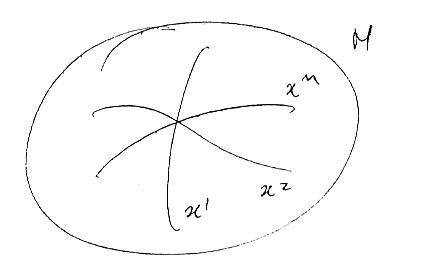
\includegraphics[width=0.75\columnwidth]{media/legame-tra-1-forma-di-poincare-cartan-e-dinamica/11-1.jpg}
  \end{minipage}
  \begin{minipage}[c]{.49\textwidth}
    $x^1,...,x^n$ coordinate locali su M\\
  \end{minipage}
\end{flushleft}

$ \eta = \eta_k (x^1, \dots , x^n) dx^k $ $ 1 $-forma differenziale su $ M $ \\
L'operazione di differenziazione, notoriamente definita nelle funzioni $ f : M \rightarrow \mathbb{R} $

\begin{equation} \label{eq:poin_cart_1}
  df = \frac{\partial f}{\partial x^k} \, (x^1, \dots , x^n) dx^k
\end{equation}

si estende nella $ 1 $-forma differenziale nel modo seguente

\begin{equation} \label{eq:poin_cart_2}
  d\eta = \frac{\partial \eta_{k}}{\partial x^r} \, dx^r \wedge dx^k = \frac{1}{2} \left( \frac{\partial \eta_{k}}{\partial x^r} - \frac{\partial \eta_{r}}{\partial x^k} \right) dx^r \otimes dx^k
\end{equation}

Osserviamo l'intrinsecità dell'operazione. Sia $ x'^k = x'^k (x^1, \dots , x^n) $ un cambiamento di coordinate

\begin{equation*}
  \begin{split}
    \eta &= \eta_k dx^k = \eta_k \frac{\partial x^k}{\partial x'^r} dx'^r \overset{def}{=} \eta'_r dx'^r\\
    &\Rightarrow \eta'_r=\eta_k \frac{\partial x^k}{\partial x'^r}
  \end{split}
\end{equation*}

Ora

\begin{equation*}
  \begin{split}
    & \left( \frac{\partial\eta'_k}{\partial x'^r} - \frac{\partial\eta'_r}{\partial x'^k} \right) dx'^r \otimes dx'^k = \\ 
    &= \left[ \frac{\partial}{\partial x'^r} \left( \eta_s \frac{\partial x^s}{\partial x'^k} \right) - \frac{\partial}{\partial x'^k} \left( \eta_s \frac{\partial x^s}{\partial x'^r} \right) \right] \frac{\partial x'^r}{\partial x^v} dx^v \otimes \frac{\partial x'^k}{\partial x^w} dx^w=\\
    &=\left[ \frac{\partial \eta_s}{\partial x'^r} \frac{\partial x^s}{\partial x'^k} + \cancel{\eta_s\frac{\partial ^2 x^s}{\partial x'^r\partial x'^k}} - \frac{\partial \eta_s}{\partial x'^k} \frac{\partial x^s}{\partial x'^r} + \cancel{\eta_s\frac{\partial ^2 x^s}{\partial x'^k\partial x'^r}} \right] \frac{\partial x'^r}{\partial x^v} dx^v \otimes \frac{\partial x'^k}{\partial x^w} dx^w=\\
    &= \left[ \frac{\partial x'^r}{\partial x^v} \frac{\partial \eta_s}{\partial x'^r} \frac{\partial x^s}{\partial x'^k} \frac{\partial x'^k}{\partial x^w} - \frac{\partial x'^k}{\partial x^w} \frac{\partial \eta_s}{\partial x'^k} \frac{\partial x^s}{\partial x'^r} \frac{\partial x'^r}{\partial x^v} \right] dx^v \otimes dx^w=\\
    &= \left[ \frac{\partial \eta_s}{\partial x^v} \delta^s w - \frac{\partial \eta_s}{\partial x^w} \delta^s v \right] dx^v \otimes dx^w = \\
    &= \left( \frac{\partial \eta_w}{\partial x^v} - \frac{\partial \eta_v}{\partial x^w} \right) dx^v \otimes dx^w
  \end{split}
\end{equation*}

e questo mostra che l'algoritmo di calcolo dato dalla ($ \ref{eq:poin_cart_2} $) è lo stesso in tutti i sistemi di ambiente, ovvero che l'operazione ($ \ref{eq:poin_cart_2} $) è intrinseca.\\
(Per esercizio provare che non è intrinseca l'operazione $ \frac{1}{2} \left( \frac{\partial \eta_{k}}{\partial x^r} + \frac{\partial \eta_{r}}{\partial x^k} \right) dx^r \otimes dx^k $).\\
In particolare, si osservi che, per un'arbitraria funzione $f$

\begin{equation*}
  \begin{split}
    ddf&=d \left( \frac{\partial f}{\partial x^k}dx^k\right) = \left( \frac{\partial}{\partial x^r} \frac{\partial f}{\partial x^k} - \frac{\partial}{\partial x^k} \frac{\partial f}{\partial x^r} \right) dx^r \otimes dx^k = 0
  \end{split}
\end{equation*}

\begin{flushright}
(vedi nota\footnote{Il termine $dF$ nella \textit{condizione di Lie} non influenza la dinamica ($ddF$ è autenticamente nullo)})
\end{flushright}

Applichiamo queste condizioni alla $ 1 $-forma differenziale di Poincaré-Cartan

\begin{equation*}
  \begin{split}
    \theta &= P_i dq^i - H (t, q^r, P_r) dt\\
    d\theta &= dP_i \wedge dq^i - \frac{\partial H}{\partial q^r} dq^r \wedge dt - \frac{\partial H}{\partial P_r} dP_r \wedge dt
  \end{split}
\end{equation*}

% INIZIO PAGINA 12

Ordinando gli elementi della base delle $ 1 $-forme differenziali nel modo seguente: $ \{ dt, dq^1, \dots , dq^n, dP_1, \dots , dP_n \} $, la matrice (antisimmetrica) rappresentabile dalla $ 2 $-forma differenziale $ d \theta $ è

\begin{equation*}
  \renewcommand\arraystretch{3}
  \begin{array}{c c}
    \qquad &
    \begin{array}{c c c}
      % \hphantom{\frac{\partial H}{\partial \uline{P}}} & \hphantom{\left( - \frac{\partial H}{\partial \uline{q}} \right)^T} & \hphantom{\left( - \frac{\partial H}{\partial \uline{P}} \right)^T}\\
      dt \qquad & d \uline{q} \qquad & d \uline{P} \qquad
    \end{array}\\
    \begin{array}{c}
      dt\\
      d \uline{q}\\
      d \uline{P}
    \end{array}&
    \begin{array}{| c | c | c |}
      \hline
      0 & \left( - \frac{\partial H}{\partial \uline{q}} \right)^T & \left( - \frac{\partial H}{\partial \uline{P}} \right)^T\\
      \hline
      \frac{\partial H}{\partial \uline{q}} & 0 & I_{n \times n}\\
      \hline
      \frac{\partial H}{\partial \uline{P}} & - I_{n \times n} & 0\\
      \hline
    \end{array}
  \end{array}_{(2n + 1) \times (2n + 1)}
\end{equation*}

Esiste uno ed un solo campo vettoriale $ Z $ (con componente $ 1 $ lungo $ \frac{\partial}{\partial t} $) che ``annulla'' la $ 2 $-forma differenziale $ d\theta $; esso è il campo tale che $ Z \rfloor d \theta = 0 $ e $ \langle Z, dt \rangle =1 $. Notare che $ d\theta $ è antisimmetrica e lo spazio ha dimensione dispari $ (2n+1) $; ma $ Z $ t.c. $ Z \rfloor d \theta = 0 $ esiste certamente, e la condizione $ \langle Z, dt \rangle = 1 $ lo ``normalizza''.\\

\begin{equation*}
  Z = \frac{\partial}{\partial t} + \frac{\partial H(t,q^r,P_r)}{\partial P_k} \frac{\partial}{\partial q^k} - \frac{\partial H(t,q^r,P_r)}{\partial q^k} \frac{\partial}{\partial P_k}
\end{equation*}

matematicamente equivalente al sistema hamiltoniano

\begin{equation*}
  \begin{split}
    \frac{dt}{dt} &= 1 \\
    \frac{dq^k}{dt} &= \frac{\partial H(t,q^r,P_r)}{\partial P_k} \\
    \frac{dP_k}{dt} &= - \frac{\partial H(t,q^r,P_r)}{\partial q^k} \\
  \end{split}
\end{equation*}

\begin{flushleft}
  \begin{minipage}[c]{.5\textwidth}
    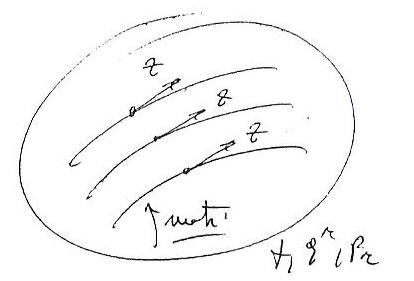
\includegraphics[width=0.75\columnwidth]{media/legame-tra-1-forma-di-poincare-cartan-e-dinamica/12-1.jpg}
  \end{minipage}
\end{flushleft}
